\documentclass [11pt, a4wide, twoside]{article}

\usepackage{verbatim}
\usepackage{times}
\usepackage{ifthen}
\usepackage{fancyhdr}
\usepackage{graphicx}
\usepackage{setspace}
\usepackage{listings}
\usepackage{tabto}
\usepackage[colorlinks,urlcolor=black,linkcolor=black,urlcolor=blue]{hyperref}
\usepackage{lastpage}
\usepackage{subfig}
\usepackage{amsmath}
\usepackage{enumerate}
\usepackage{xspace}
\usepackage{textcomp}
\usepackage[euler-digits,euler-hat-accent]{eulervm}

\newcommand{\caret}{\hspace*{0.125cm}$\hat{}$\hspace*{0.05cm}}

\lstset{
  backgroundcolor=\color{white},   % choose the background color; you must add \usepackage{color} or \usepackage{xcolor}
  basicstyle=\footnotesize\ttfamily,        % the size of the fonts that are used for the code \tiny \scriptsize
  breakatwhitespace=false,         % sets if automatic breaks should only happen at whitespace
  breaklines=true,                 % sets automatic line breaking
  captionpos=b,                    % sets the caption-position to bottom
  mathescape=true,
  commentstyle=\color{black},    % comment style
  deletekeywords={...},            % if you want to delete keywords from the given language
  escapechar=\@
  escapeinside={\%*}{*)},          % if you want to add LaTeX within your code
  extendedchars=true,              % lets you use non-ASCII characters; for 8-bits encodings only, does not work with UTF-8
  keepspaces=true,                 % keeps spaces in text, useful for keeping indentation of code (possibly needs columns=flexible)
  keywordstyle=\color{black},       % keyword style
  language=Java,                 % the language of the code
  morekeywords={*,...},            % if you want to add more keywords to the set
  numbers=none,                    % where to put the line-numbers; possible values are (none, left, right)
  numberstyle=\tiny, % the style that is used for the line-numbers
  rulecolor=\color{black},         % if not set, the frame-color may be changed on line-breaks within not-black text (e.g. comments (green here))
  showspaces=false,                % show spaces everywhere adding particular underscores; it overrides 'showstringspaces'
  showstringspaces=false,          % underline spaces within strings only
  showtabs=false,                  % show tabs within strings adding particular underscores
  stepnumber=2,                    % the step between two line-numbers. If it's 1, each line will be numbered
  stringstyle=\color{black},     % string literal style
  tabsize=2,                       % sets default tabsize to 2 spaces
  xleftmargin=.25in,
  title=\lstname                   % show the filename of files included with \lstinputlisting; also try caption instead of title
}

% solution switch
\newboolean{showsolution}
\setboolean{showsolution}{true} 

%layout
\topmargin      -5.0mm
\oddsidemargin  6.0mm
\evensidemargin -6.0mm
\textheight     215.5mm
\textwidth      160.0mm
\parindent      1.0em
\headsep        10.3mm
\headheight     12pt
\lineskip       1pt
\normallineskip 1pt

%header
\lhead{SMA: Software Modeling and Analysis\\A2020}

\rhead{Prof. Dr. Oscar Nierstrasz\\Pascal Gadient, Pooja Rani}

\lfoot{page \hspace{0.03cm} \thepage \hspace{0.11cm} of \hspace{0.09cm} \pageref*{LastPage}}
\rfoot{16 December 2020}
%\rfoot{\today}
\cfoot{}

\renewcommand{\headrulewidth}{0.1pt}
\renewcommand{\footrulewidth}{0.1pt}

\def\xexercise{\fontsize{12}{10}\fontseries{bx}\selectfont}
\def\xnormal{\fontseries{m}\fontshape{n}\selectfont}

\newcounter{exnum}
\newcommand{\exercise}[1]{%
	{\addtocounter{exnum}{1}\vskip 0.8cm{\xexercise \noindent Exercise \arabic{exnum} -- #1} \xnormal} \vskip 0.3cm}
\newcommand{\aufgabe}[1]{
	{\addtocounter{exnum}{1}\vskip 0.8cm{\xexercise \noindent Aufgabe \arabic{exnum} - #1} \xnormal} \vskip 0.3cm}

%enumeration
\newenvironment{myitemize}{%
     \begin{itemize}
     \setlength{\itemsep}{0cm}}
     {\end{itemize}}

\newenvironment{myenumerate}{%
	\renewcommand{\labelenumi}{\alph{enumi})}
	\renewcommand{\labelenumii}{\arabic{enumii})}
     \begin{enumerate} \setlength{\itemsep}{0cm}}
     {\end{enumerate}}


%solution
\ifthenelse{\boolean{showsolution}}
   {  \newcommand{\solution}[1]{
   	\noindent\underline{\textcolor{red}{\textbf{Answer:}}}\\[2mm]
   	 \textsl{\textcolor{red}{#1}}
	 \vspace{10pt}
	 \normalsize
	}
  }
  {  \newcommand{\solution}[1]{} }


\pagestyle{fancy}


\newcommand{\ie}{\emph{i.e.},\xspace}
\newcommand{\eg}{\emph{e.g.},\xspace}
\newcommand{\etc}{\emph{etc.}\xspace}

\graphicspath{{./figures/}}

\begin{document}

\section*{\ifthenelse{\boolean{showsolution}}{Solution }{}Software Modeling and Analysis - Exam}
Given Name:\tabto{4cm}\rule{100pt}{0.5pt}\\[1mm]\\
Family Name:\tabto{4cm}\rule{100pt}{0.5pt}\\[1mm]\\\\
Matriculation Number:\tabto{4cm}\rule{100pt}{0.5pt}\\[1mm]\\
\rule{\textwidth}{1pt}\\[1mm]
\begin{center}
\textbf{Please read this page carefully and fill in your name right away!}
\end{center}
\vspace{1cm}
Examination date:\tabto{4.5cm}Wednesday, 16 December 2020\\
Version:\tabto{4.5cm}1.0\\\\
Time:\tabto{4.5cm}60 minutes\\
Total points:\tabto{4.5cm}60 (one point requires about 1 minute of work)\\
Number of exercises:\tabto{4.5cm}6\\
Allowed materials:\tabto{4.5cm}a single ink-based pen (no pencil)\\\\

\noindent Please remember:
\begin{enumerate}
\item Some exercises are split over more than one page. Please quickly skim through all exercises first, before you proceed with the exam.
\item Don't forget to answer every aspect of a question, \ie \underline{reply to every question mark}.
\item If you don't know something don't waste any time, go ahead and try to solve those questions at the end.
\item You are expected to answer each question concisely (brief and precise).
%\item If you need more blank space for your answers, please use the back of your pages, and \underline{clearly state} to which question your answer relates.
\item Please pay attention that your handwriting is easily readable for other people.
\item Cheating irreversibly leads to the grade 1.
\end{enumerate}
%\rule{\textwidth}{1pt}

\newpage

\exercise{General Questions (15 points $\mid$ approx. 15 minutes)}
\noindent Answer the the following questions:
\begin{myenumerate}
\item Which class represents the root of GT's class hierarchy? \textbf{(1~point)}
\solution{ProtoObject}
\ifthenelse{\boolean{showsolution}}{}{\vspace{1.5cm}}

\item Where can you find a meta-model in Pharo? \textbf{(1~point)}
\solution{Metaclasses are a typical manifestation of the meta-model concept. Moreover, the class "Class" can be considered a meta-model for class instances.}
\ifthenelse{\boolean{showsolution}}{}{\vspace{1.5cm}}

\item What is the benefit of using a meta-model? \textbf{(1~point)}
\solution{A meta-model improves the modularity and portability of a design due to better separation of concerns.}
\ifthenelse{\boolean{showsolution}}{}{\vspace{1.5cm}}

\item Which two reflection abilities do you know? What is the difference between both? \textbf{(2~points)}
\solution{Introspection (reading) and intercession (reading and writing). The latter also supports changes of state.}\vspace{3cm}

\item Briefly explain the concept of static, dynamic, and hybrid code analysis \underline{each in one sentence}. \textbf{(3~points)}
\solution{Static analysis: analysis of (source) code \\ Dynamic analysis: analysis of program execution \\ Hybrid analysis: a combination of both}
\ifthenelse{\boolean{showsolution}}{}{\vspace{4.5cm}}

\item In what sense is GT a live programming environment?~\textbf{(1~point)}
\solution{Everything changed in the GT environment will apply immediately to the whole system with all the consequences.}
\ifthenelse{\boolean{showsolution}}{}{\vspace{1.5cm}}

\item Which threats may arise due to users unrestricted access to GT's system classes? \textbf{(1~point)}
\solution{The system state may become corrupted due to flawed user input. Unexpected or wrong results might occur.}
\ifthenelse{\boolean{showsolution}}{}{\vspace{1.5cm}}

\newpage

\item What is the syntax for a comment in Smalltalk? \textbf{(1~point)}
\solution{Comments are enclosed by the double quote character, \eg "I am a comment."}
\ifthenelse{\boolean{showsolution}}{}{\vspace{1.5cm}}

\item What is the difference between a string (\texttt{\textquotesingle HelloWorld\textquotesingle}) and a symbol (\texttt{\#HelloWorld})? \textbf{(2~points)}
\solution{A symbol is unique, wheras a string is not.}
\ifthenelse{\boolean{showsolution}}{}{\vspace{3cm}}

\item Provide one argument for the use of GT for (software) prototyping \underline{and} one against it. \textbf{(2~points)}
\solution{Yes, because it supports developers in efficiently crafting a solution.\\No, because Smalltalk is not very common compared to mainstream languages such as Java or C, and it is hard to find people to collaborate with on a global project.}
\ifthenelse{\boolean{showsolution}}{}{\vspace{3cm}}
\end{myenumerate}

\newpage

\exercise{Smalltalk Coding (10 points $\mid$ approx. 10 minutes)}
\noindent Answer the following questions:
\begin{myenumerate}
\item What does the code below do? \textbf{(2~points)}
\begin{lstlisting}
(((SystemNavigation default allClasses collect: [ :eachClass |
	eachClass -> eachClass classDepth]) sorted:[ :a :b |
		a value > b value ]) asOrderedDictionary) keys first
\end{lstlisting}
\solution{The code finds the class with the longest inheritance chain among all Smalltalk classes in the GT programming environment.}
\ifthenelse{\boolean{showsolution}}{}{\vspace{3cm}}

\item Fill in the blanks to complete the method that returns all method names in GT. \textbf{(4~points)}\\
\begin{lstlisting}
(( ______________________ ________________ ________________


	collect:	[ _______________ | _______________ _________ ])


	sorted:		[ ____________ | ____________ ]).
\end{lstlisting}
\solution{
((SystemNavigation default allMethods\\
\hspace*{0.5cm}collect: [ :eachMethod \textbar~eachMethod name])\\
\hspace*{0.5cm}sorted:[ :a :b \textbar~a \textless~b ]).}

\item When do you need to use the \texttt{\textless gtView\textgreater} pragma? How do you use it? \textbf{(2~points)}
\solution{The pragma declares the method as ``viewable'' in the GT inspector. Hence, we need to set it if we would like to create a custom view in the GT inspector. The pragma must appear after the method declaration but before the method body.}
\ifthenelse{\boolean{showsolution}}{}{\vspace{4cm}}

\item What is a ``live document''? Which problem frequently found in traditional code documentation does it solve? \textbf{(2~points)}
\solution{A live document is a document that contains executable code. As a result, it can update itself based on the results of the contained code.\\Outdated or inconsistent documentation is a serious problem. Live documents avoid discrepancies in the documentation by design, because they evolve with the code.}
\ifthenelse{\boolean{showsolution}}{}{\vspace{3cm}}
\end{myenumerate}

\newpage

\exercise{Dynamic Smalltalk Coding (8 points $\mid$ approx. 8 minutes)}
Assume a \texttt{String} instance contains the following message implementation.\\\\
\texttt{\hspace*{1.0cm}addMethod: aString\\
\hspace*{1.5cm}self class compile: \\
\hspace*{2.0cm}aString, \textquotesingle: aString\textquotesingle, String cr, \textquotesingle\caret~aString size.\textquotesingle.}\\

\begin{myenumerate}
\item What does the method \texttt{compile:} do? \textbf{(2~points)}
\solution{It compiles the provided string and adds a reference to the compiled code to the instance's method dictionary, if the string contains code for a method.}
\ifthenelse{\boolean{showsolution}}{}{\vspace{3cm}}

\item Assume\\
\hspace*{0.5cm}\texttt{s := String new addMethod: \textquotesingle myMethod\textquotesingle.}\\
has been executed in the Playground on such a modified \texttt{String} instance. What is the content of the \texttt{myMethod:} implementation? \textbf{(3~points)}
\solution{myMethod: aString\\
\caret~aString size.}
\ifthenelse{\boolean{showsolution}}{}{\vspace{3cm}}

\item Assume\\
\hspace*{0.5cm}\texttt{s myMethod: \textquotesingle Hello World\textquotesingle.}\\
has been subsequently executed in the Playground. What is the returned result? \textbf{(1~point)}
\solution{11 (a SmallInteger object)}
\ifthenelse{\boolean{showsolution}}{}{\vspace{2cm}}

\item Name one benefit of dynamic coding and explain why it is a benefit. \textbf{(2~points)}
\solution{Methods can be manipulated programmatically. This is a huge benefactor for maintenance and automatization, \eg methods can be changed without restarting the execution environment, and hot patches to running code can be applied without any human interaction.}
\ifthenelse{\boolean{showsolution}}{}{\vspace{3cm}}
\end{myenumerate}

\newpage

\exercise{Software Metrics and Analyses (8 points $\mid$ approx. 8 minutes)}
Consider the code in \autoref{e05-listing} and answer the questions below.

\begin{figure}[thp]
\centering
\begin{tabular}{c}
\definecolor{violet}{RGB}{255,0,0}
\lstset{language=}
\begin{lstlisting}
int gcd(int a, int b) {
	if (a == 0) { 
		return b; 
	}
	
	while (b != 0) {
		if (a > b) {
			a = a - b;
		} else {
			b = b - a; 
	 	}
	}
	
	return a;
}
\end{lstlisting}
\end{tabular}
\vspace{-0.4cm}
\caption{Sample Java method}
\label{e05-listing}
\end{figure}

\begin{myenumerate}
\item Provide the common cyclomatic complexity formula we used in the lecture and explain each parameter of it. \textbf{(3~points)}
\solution{The formula is defined as $M = E - N + 2*P$, whereas $M$ represents the resulting metric,\ie the complexity value, $E$ represents the number of edges of the CFG (possible different instruction flows), $N$ represents the number of nodes in the CFG (instructions), and $P$ represents the number of connected components ($P = 1$ for the analysis of a method).}
\ifthenelse{\boolean{showsolution}}{}{\vspace{10cm}}

\begin{center}
\textbf{\textit{You will find more questions on the next page.}}
\end{center}

\newpage

\item Draw the regular (non-interval) CFG for the code shown in~\autoref{e05-listing}. \textbf{(4~points)}
\solution{\begin{figure*}[ht!]\centering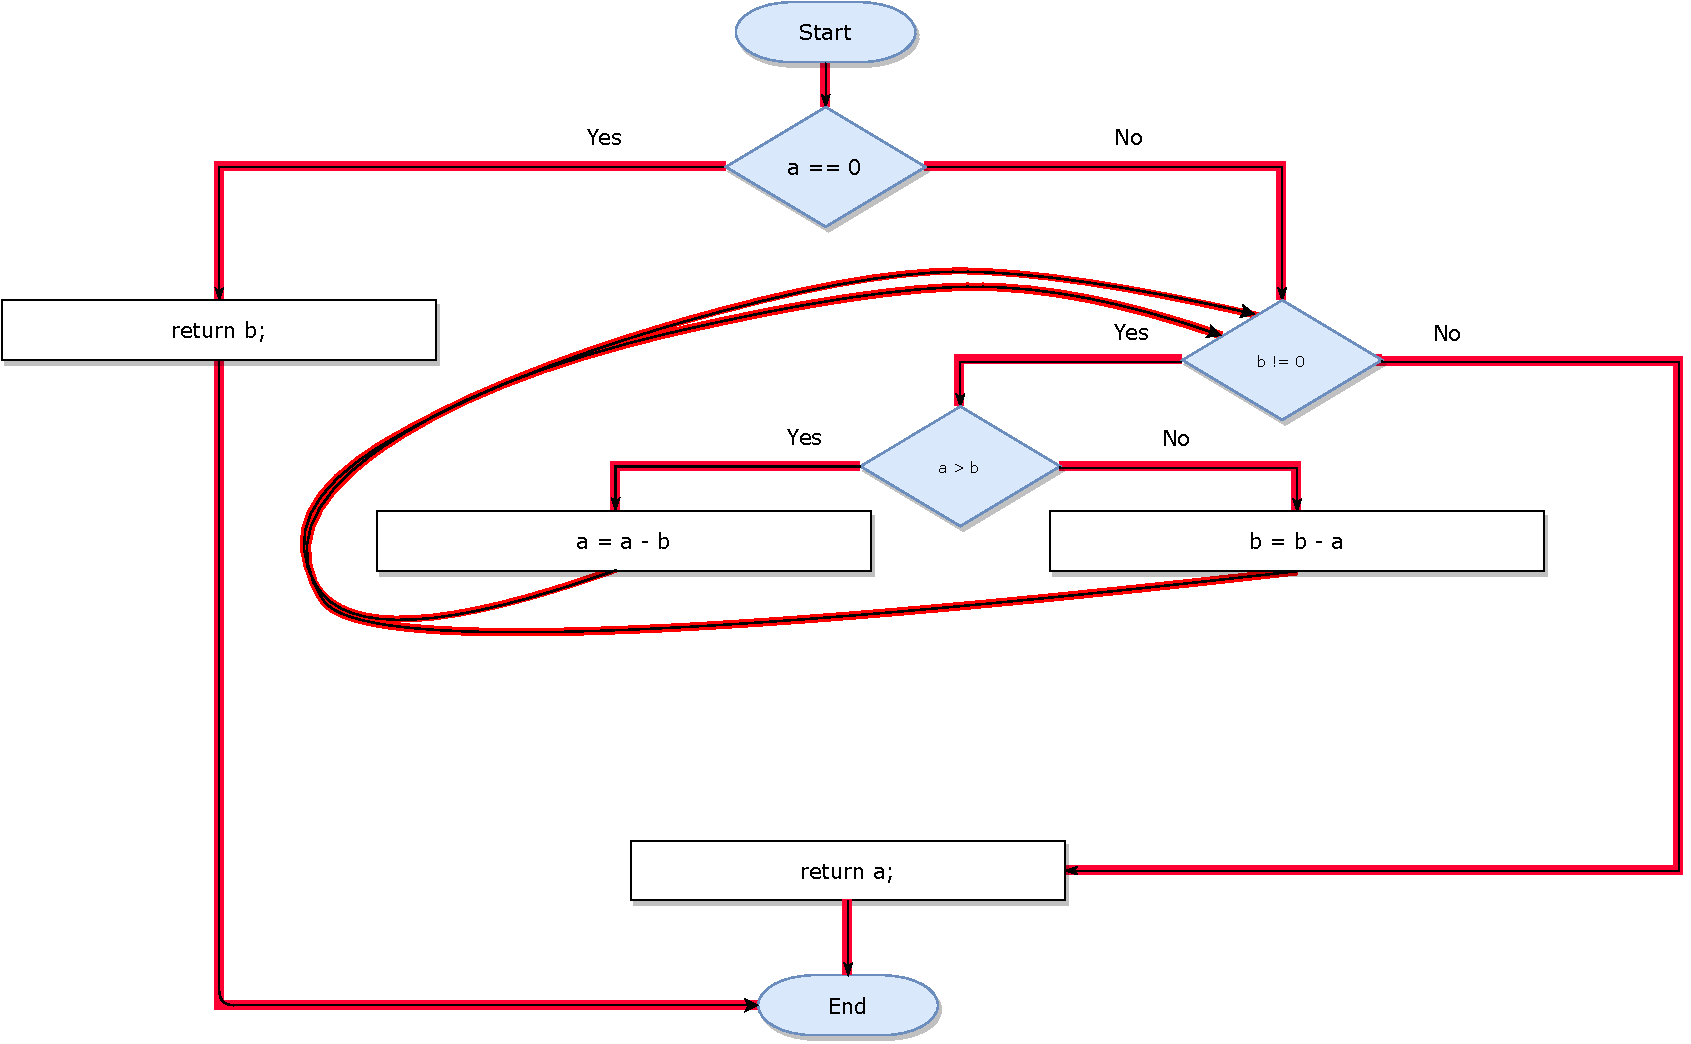
\includegraphics[scale=0.55,trim={0.75cm 0.75cm 0.75cm 0.75cm}]{figures/4b.pdf}\end{figure*}}
\ifthenelse{\boolean{showsolution}}{}{\vspace{19cm}}

\item What is the cyclomatic complexity of the code in~\autoref{e05-listing}? \textbf{(1~point)}
\solution{4}
\ifthenelse{\boolean{showsolution}}{}{\vspace{1cm}}

\end{myenumerate}

\newpage

\exercise{Test Code Smells (10 points $\mid$ approx. 10 minutes)}
Consider the code in \autoref{e06-listing} and answer the questions below.

\begin{figure}[thp]
\centering
\begin{tabular}{c}
\definecolor{violet}{RGB}{255,0,0}
\lstset{language=}
\begin{lstlisting}
public class Compute {
	public static String mod(int number, int divisor) {
		if (number < divisor) {
			return number; 
		} else {
			number -= divisor;
			return mod(number, divisor);
		}
	}
}

public void testMod() {
	// only run during night
	int currentHour = InternetTime.getCurrent(Calendar.HOUR);
	if (currentHour > 20) {
		int resultWithRemainder = Compute.mod(13,7);
		assertEquals(6, resultWithRemainder);
	}
}
\end{lstlisting}
\end{tabular}
\vspace{-0.2cm}
\caption{Sample (Java) code with a JUnit test case}
\label{e06-listing}
\end{figure}

\begin{myenumerate}
\item What does the static method compute? \textbf{(1~point)}
\solution{It computes the modulo operation.}
\ifthenelse{\boolean{showsolution}}{}{\vspace{2cm}}

\item The code of the \underline{static method} contains multiple flaws. Identify one flaw and provide a pair of integer numbers that break the implementation, \ie lead to exceptions, errors, or wrong results. Provide the two numbers you found (\ie a \texttt{number} and a \texttt{divisor}) \underline{and} briefly explain what the problem is. \textbf{(2~points)}
\solution{The code suffers from stack overflow errors when a divisor of 0 is provided, and it leads to stack overflow errors or broken results when the input contains negative integers. Because the bounds check is faulty, the recursion never stops (stack overflow) or skips inappropriately (negative numbers).}
\ifthenelse{\boolean{showsolution}}{}{\vspace{5.75cm}}

\newpage

\item Write a test case for the flaw you just found. \textbf{(3~points)}
\solution{
The provided solutions must be reasonable. They should exploit the discovered flaw.
Two examples:\\\\
public void testModZero() \{\\
\hspace*{0.5cm}Assertions.assertThrows(StackOverflowException.class, () -\textgreater~\{\\
\hspace*{1.0cm}resultWithRemainder = Compute.mod(13,0);\\
\hspace*{0.5cm}\});\\
\}\\\\
public void testModNegativeNumber() \{\\
\hspace*{0.5cm}int resultWithRemainder = Compute.mod(-5,7);\\
\hspace*{0.5cm}assertEquals(2, resultWithRemainder);\\
\}
}
\ifthenelse{\boolean{showsolution}}{}{\vspace{7cm}}

\item Do you find a \emph{test code smell}? If yes, where do you find it, and what is problem it could introduce? \textbf{(2~points)}
\solution{Yes, the (i) use of ``testMod'' as test name. This misleads developers, because it does not comprehensively test the method and is too generic. (ii) An external resource is used within the test. Depending on its availability the test results could differ. A (iii) conditional in the test. This complicates the interpretation of results, because some code paths might not be tested.}
\ifthenelse{\boolean{showsolution}}{}{\vspace{6cm}}

\item Is \emph{Feature Envy} considered a \emph{code smell} or a \emph{test code smell}? \textbf{(1~point)}
\solution{It is a code smell.}
\ifthenelse{\boolean{showsolution}}{}{\vspace{2cm}}

\item Is \emph{Assertion Roulette} considered a \emph{code smell} or a \emph{test code smell}? \textbf{(1~point)}
\solution{It is a test code smell.}
\ifthenelse{\boolean{showsolution}}{}{\vspace{2cm}}
\end{myenumerate}

\newpage

\exercise{Fuzz Testing (9 points $\mid$ approx. 9 minutes)}
Please answer the following questions:
\begin{myenumerate}
\item Briefly explain each of the terms \emph{black box fuzzing}, \emph{white box fuzzing}, and \emph{grey box fuzzing}. \textbf{(3~points)}
\solution{Fuzzing is the process of creating new or altered input and then monitoring apps given the generated input.\\Black box fuzzing: fuzzer knows nothing about the target application and its input.\\
White box fuzzing: fuzzer leverages data from program analysis and constraint solving to improve the quality of the results.\\ 
Grey box fuzzing: fuzzer has some knowledge about the program, \ie it is a combination of black and white box fuzzing.}
\ifthenelse{\boolean{showsolution}}{}{\vspace{5cm}}

\item Answer the following questions regarding the \texttt{zzuf} tool:\\(i) What is the purpose of the tool? \textbf{(1~point)}\\(ii) Does the tool perform a static or dynamic code analysis? \textbf{(1~point)}\\(iii) Is its output deterministic? \textbf{(1~point)}
\solution{(i) It is used to fuzz applications to find bugs or security vulnerabilities. zzuf is a transparent application input fuzzer and it can generate new input from existing data.\\(ii) It is a dynamic code analyzer, because it needs to execute the application to gather results.\\(iii) Yes, its output is deterministic.}
\ifthenelse{\boolean{showsolution}}{}{\vspace{6cm}}

\item Suppose you want to fuzz test a Smalltalk parser. What would be a suitable input string for a grey box fuzzer to start with?
\textbf{(1~points)}
\solution{Any valid Smalltalk code snippet. For example:\\
Transcript show: \textquotesingle Hello World\textquotesingle.}
\ifthenelse{\boolean{showsolution}}{}{\vspace{2cm}}

\item Suppose you use that input string. How could the input string look like after one iteration if you use a mutation-based fuzzer? Which mutation rule did you apply? \textbf{(2~points)}
\solution{Any answer is reasonable. The only requirement is that the provided code snippet must be altered and a rule must be followed (character substitutions, insertions, ..., randomness).\\\\For example:\\A rule that converts every non-letter character to a period would create this input after one iteration:\\Transcript.show...Hello.World..}
\ifthenelse{\boolean{showsolution}}{}{\vspace{2cm}}
\end{myenumerate}

\end{document}
